\section{The Moon-to-Moon Analytical Transfer Method}
The MMAT method was created to design tours between the moons of a planet such as Jupiter or
Saturn. However, Canales also showed that it could similarly be used for interplanetary transfers
by treating the planets as "moons" of the Sun. He provides detailed derivations, analyses, and
examples of the basic MMAT strategy, as well as some extensions relevant to this
investigation\cite{Canales:2021a,Canales:2021b,Canales:2022}. More specifically, the end-to-end
cislunar-Mars transfer methodology presented here uses a distant, two-burn MMAT with a plane
change. This accounts for bridging the gap between manifolds of Sun-planet CR3BP systems and the
true orbital plane inclinations of the planets.

\subsection{Methodology}
First, a departure and an arrival CR3BP arc are needed. In this investigation, the departure CR3BP
arc is either a Sun-Earth halo orbit unstable manifold trajectory or an Earth-Moon orbit unstable
manifold arc propagated with the Sun-Earth dynamics, depending on the transfer category. Either the
departure epoch or the chosen manifold arc are varied to determine the departure CR3BP arc
respectively. The arrival CR3BP arc is a Sun-Mars halo orbit stable manifold trajectory. Since an
interplanetary transfer from Earth to Mars is an outward journey, to minimize the $\Delta v$ of the
MMAT transfer, the Sun-Mars stable manifold with the smallest periapsis (relative to the Sun) is
used\cite{Canales:2021b}. (For an inward journey, say to Venus, the manifold with the largest
apoapsis is chosen.) This minimizes the Keplerian angular momentum and energy difference between
the departure and arrival CR3BP arcs.

These arcs are propagated under the CR3BP dynamics until they reach a specified distance from their
smaller primary (Earth or Mars), known as a sphere of influence (SoI). Various definitions exist,
but for the MMAT method, the SoI radius is defined as the distance for which the ratio of the
gravitational accelerations of the two primaries $d_{SoI}$ is equal to a chosen small
quantity (see \cref{eq:patchedSoI})\cite{Canales:2021b}. To ensure that the SoI encompasses most of the Lyapunov family but
also accurately represents when that body's gravitational effects can be neglected, the values of
$d_{SoI}$ in \cref{tab:SoI} are chosen, resulting in their corresponding radii. Canales provides
more details on selecting of appropriate values for $d_{SoI}$\cite{Canales:2021b}.

\begin{table}[ht]
    \centering
    \caption{MMAT sphere of influence radii of relevant CR3BP systems.}
    \begin{tabular}{|c|c|c|}
        \hline
        \textbf{CR3BP System}   &   \boldmath$d_{SoI}$  &   \boldmath$r_{SoI}$  \\  \hline
        Sun-Earth               &   $2.5\times10^{-4}$  &   $0.09877$           \\  \hline
        Sun-Mars                &   $1\times10^{-4}$    &   $0.05375$           \\  \hline
    \end{tabular}
    \label{tab:SoI}
\end{table}

Once the CR3BP arc has reached the edge of the SoI, it can be treated as a 2BP trajectory with the
Sun as its focus (refer to the patched 2BP-CR3BP model introduced in Section 2.4.1). The
barycentric rotating frame state that intersects the SoI is transformed to a heliocentric Ecliptic
J2000 inertial frame state using the procedure outlined in Section 2.5.2. The resulting inertial
state now defines a Keplerian heliocentric ellipse, the path for either the departure or arrival
conic arc. \cref{eq:inclination}-\cref{eq:radialvelocity} can be used to retrieve the equivalent
Keplerian orbital elements.

In the distant, two-burn MMAT strategy, the first maneuver is placed at the periapsis of the
departure conic. Given that the true anomaly $\theta=0$ at periapsis,
\cref{eq:eccentricanomaly}-\cref{eq:velocityvector} are used to compute the inertial state at
periapsis while \cref{eq:meananomaly} and \cref{eq:Keplersequation} are used to compute the
time-of-flight along the departure conic:
\begin{equation}
    TOF_{d}=\mathbb{P}_{d}-(t-t_{p}),
    \label{eq:departureTOF}
\end{equation}
where $\mathbb{P}_{d}$ is the period of the departure conic and $(t-t_{p})$ is the time since
periapsis of the inertial SoI state.

As mentioned previously, a bridge arc is needed to connect the departure and arrival conic arcs,
with a maneuver at both ends. The distant, two-burn MMAT bridge arc has the same periapsis radius
as the departure conic arc and the same apoapsis as the arrival conic arc. These values form a
bridge ratio which can then be used to compute the semimajor axis and eccentricity of the bridge
conic:
\begin{equation}
    \mathcal{P}_{b}=\frac{r_{p_{b}}}{r_{a_{b}}}=\frac{1-e_{b}}{1+e_{b}},
    \label{eq:bridgeratio}
\end{equation}
\begin{equation}
    e_{b}=\frac{1-\mathcal{P}_{b}}{1+\mathcal{P}_{b}},
    \label{eq:bridgeeccentricity}
\end{equation}
\begin{equation}
    a_{b}=\frac{r_{p_{b}}}{1-e_{b}}.
    \label{eq:bridgesemimajoraxis}
\end{equation}
The remaining three angles of the bridge conic ($i$, $\Omega$, $\omega$) are identical to those of
the departure conic, implying that the bridge arc lies in the same plane as the departure conic
arc. Since only the semimajor axis and eccentricity change between the departure and bridge conics,
this first maneuver is tangential to the motion (only changing the energy) at periapsis and can be
calculated by the difference in the velocity states at periapsis.

The non-coplanar MMAT methodology revolves around the following analytical constraint derived by
Canales\cite{Canales:2021b}:
\begin{quote}
    As long as the geometrical properties of two conics located in different planes fulfill the
    inequality constraint represented by
    \begin{equation}
        a_{a}(1-e_{a})\leq\frac{a_{b}(1-e_{b}^{2})}{1+e_{b}\cos(\theta_{b_{int}}+n\pi)}\leq a_{a}(1+e_{a}),\text{ being }n=0,1,
        \label{eq:MMAT}
    \end{equation}
    either one of the two conics can be reoriented such that they intersect in space. Consequently,
    the ideal phase of the arrival [planet] at arrival, $\theta_{5_{Mars}}$, for the moon-to-moon
    transfer to occur is obtained considering that the departure epoch, $\theta_{0_{Earth}}$, is
    fixed.
\end{quote}
In this constraint, $\theta_{5_{Mars}}$ and $\theta_{0_{Earth}}$ correspond to $T_{0}$ and $T_{5}$
in \cref{fig:MMAT}. This figure is a schematic of the distant, two-burn MMAT transfer with a plane
change, where the departure and bridge conics are on the same plane but the arrival conic is not.
With the semimajor axes and eccentricities of the bridge and arrival arcs already determined, the
only value still needed for \cref{eq:MMAT} is $\theta_{b_{int}}$, the bridge conic true anomaly at
the bridge-arrival conic intersection location ($T_{3}$ in \cref{fig:MMAT}):
\begin{equation}
    \theta_{b_{int}}=u_{b}-\omega_{b},
    \label{eq:bridgeintersect}
\end{equation}
\begin{equation}
    \sin u_{b}=\frac{\sin(\pi-i_{a})\sin\Delta\Omega}{\sin\psi},
    \label{eq:bridgesinu}
\end{equation}
\begin{equation}
    \cos u_{b}=\frac{\frac{\sin i_{a}\cos\Delta\Omega}{\cos i_{b}}-\cos\psi\tan i_{b}}{\sin\psi},
    \label{eq:bridgecosu}
\end{equation}
\begin{equation}
    \cos\psi=\cos i_{a}\cos i_{b}+\sin i_{a}\sin i_{b}\cos\Delta\Omega,
\end{equation}
where $\Delta\Omega=\Omega_{a}-\Omega_{b}$. Note that the value of $n$ used to satisfy the
inequality defines the orientation of the bridging conic and will be used later to properly orient
the arrival conic. The center of the inequality in \cref{eq:MMAT} is the intersection distance from
the Sun:
\begin{equation}
    r_{int}=\frac{a_{b}(1-e_{b}^{2})}{1+e_{b}\cos(\theta_{b_{int}}+n\pi)}=\frac{a_{a}(1-e_{a}^{2})}{1+e_{a}\cos(\theta_{a_{int}}+o\pi)}, \text{ being }o=0,1,
    \label{eq:intersect}
\end{equation}

Unfortunately, if the arrival conic arc is not in the same plane as the orbital plane of the
arrival planet, $i_{a}$ and $\Omega_{a}$ cannot be determined prior to the MMAT phasing (yet to
come). As a result, the arrival phasing needs to be iteratively targeted, making this approach now
only semi-analytical. For an initial guess to check the MMAT constraint in \cref{eq:MMAT}, the
inclination and RAAN of the arrival planet's orbital plane are used.

\begin{figure}[ht]
    \centering
    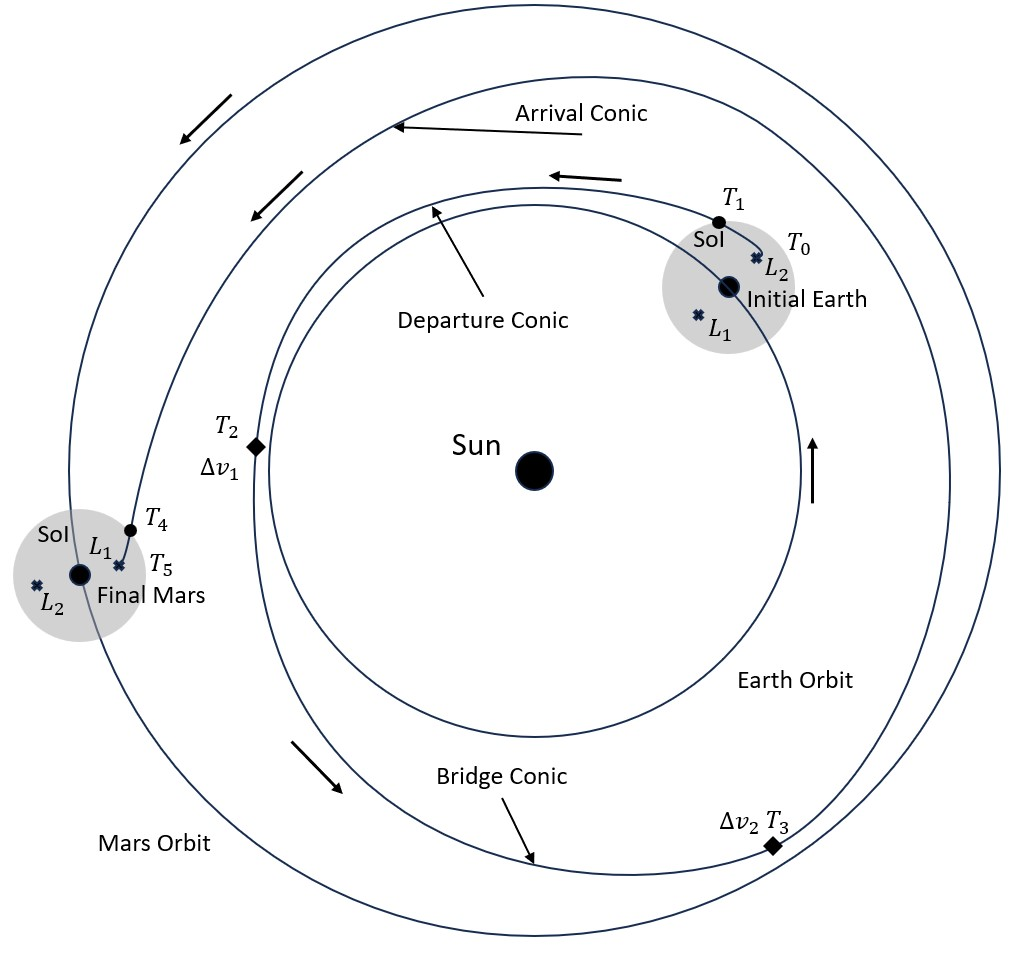
\includegraphics[width=0.75\textwidth]{figures/MMAT.jpg}
    \caption{Representation of the distant, two-burn MMAT with a plane change (adapted from Canales\cite{Canales:2021b}).}
    \label{fig:MMAT}
\end{figure}

The arrival conic true anomaly at the intersection is computed similarly from $r_{int}$, with the
caveat that it is dependent on the arrival phasing and needs to be targeted:
\begin{equation}
    \theta_{a_{int}}=2\pi o+(-1)^{o}\arccos(\frac{\frac{a_{a}(1-e_{a}^{2})}{r_{int}}-1}{e_{a}}),\text{ being }o=0,1.
    \label{eq:arrivalintersect}
\end{equation}
For every feasible $\theta_{b_{int}}$, there are then two possible phasing solutions
($\theta_{a_{int}}$) that correspond to the two arrival ellipse orientations ($\omega_{a}$) that
intersect the bridge ellipse at the line of nodes. A schematic representing these two orientations
is shown in \cref{fig:orientation}, where the dashed part of the ellipses are under the $XY$-plane
and the arrows show the direction of motion along each ellipse. The angles for the orientation are
calculated similarly to before:
\begin{equation}
    \omega_{a}=u_{a}-(\theta_{a_{int}}+n\pi),
    \label{eq:arrivalperiapse}
\end{equation}
\begin{equation}
    \sin u_{a}=\frac{\sin i_{b}\sin\Delta\Omega}{\sin\psi},
    \label{eq:arrivalsinu}
\end{equation}
\begin{equation}
    \cos u_{a}=\cos\Delta\Omega\cos u_{b}+\sin\Delta\Omega\sin u_{b}\cos i_{b}.
    \label{eq:arrivalcosu}
\end{equation}

\begin{figure}[ht]
    \centering
    \includegraphics[width=0.9\textwidth]{figures/orientation.jpg}
    \caption{Representation of the two feasible arrival ellipse orientations. The top images are $XY$-plane views while the bottom are $XZ$-plane views.}
    \label{fig:orientation}
\end{figure}

\cref{eq:arrivalperiapse} is dependent on the orientation of the arrival CR3BP arc, which in turn
depends on a properly phased arrival. Therefore, to solve for the proper phasing and orientation,
an iterative Newton-Raphson differential corrections scheme is applied:
\begin{equation}
    \Xbar=\begin{bmatrix}   \theta_{b_{int}}    &   \theta_{4_{Mars}}   &   \theta_{a_{int}}    \end{bmatrix}^{T},
    \label{eq:MMATfreevar}
\end{equation}
\begin{equation}
    \Fbar(\Xbar)=\rbar_{a}-\rbar_{b},
    \label{eq:MMATconst}
\end{equation}
where $\theta_{4_{Mars}}$ corresponds to Mars' true anomaly when the trajectory intersects the Mars
SoI. For an initial guess:
\begin{equation}
    \theta_{4_{Mars}}=\arctan(\cos i_{Mars}\tan\Omega_{Mars})+\omega_{a}+\theta_{a}-(\Omega_{Mars}+\omega_{Mars}+\theta_{Mars_{J2000}})-\arctan(\frac{y_{4}}{|x_{4}|}),
    \label{eq:arrivalepoch}
\end{equation}
where $\theta_{a}$ is the true anomaly of the arrival conic at the SoI intersection,
$\theta_{Mars_{J2000}}$ is Mars' true anomaly when the J2000 inertial frame is defined, and $x_{4}$
and $y_{4}$ are the rotating frame coordinates of the trajectory at the SoI intersection. For this
targeting problem, the $DF$ Jacobian matrix is determined using the central difference method (see
Section 3.1.3).

Once $\Xbar$ has been solved, these true anomaly angles can be used to compute the Cartesian
inertial states at each location and the times-of-flight of each segment as was done for the
departure conic arc. At the intersection of the bridge and arrival conics, the second maneuver
applies an inclination change on top of the energy change so it is not tangential like the first
burn. This $\Delta v$ can still be calculated from the difference in the velocity states at the
intersection.

The MMAT transfer between the Sun-Earth CR3BP arc and the Sun-Mars CR3BP arc is now completed. The
trajectory should be position-continuous throughout, with a maneuver at the beginning and end of
the bridge arc to account for the velocity discontinuities. For every feasible $\theta_{b_{int}}$,
there will be two corresponding $\theta_{a_{int}}$ that provide transfers. These two solutions will
have different maneuver costs and times-of-flight. By continuing in the departure epoch or the
chosen manifold arc as discussed, a family of MMAT solutions can be obtained and compared.

\subsection{Example}
What follows is an example MMAT family between a Sun-Earth CR3BP northern halo orbit at a Jacobi
constant of $3.0008189$ and a Sun-Mars CR3BP northern halo orbit at a Jacobi constant of
$3.0001857$. Each transfer in the family starts at a different initial epoch, each day in an Earth
year. These initial epochs correspond to $\theta_{0_{Earth}}$ values (which spans
0\textdegree-360\textdegree in a year). All of the trajectories use the same departure CR3BP arc,
which is the Sun-Earth halo unstable manifold with the largest apoapsis, shown in
\cref{fig:MMATSE}. Similarly, all of the trajectories use the same Sun-Mars halo stable manifold
with the smallest periapsis as the arrival CR3BP arc, shown in \cref{fig:MMATSM}. In both figures,
the trajectory is propagated and displayed to the edge of the sphere of influence. In between, the
departure and arrival conic arcs are determined by the osculating Keplerian orbital elements when
the manifolds reach their respective SoIs and the bridge conic arc joins them as described above.

\begin{figure}[ht]
    \centering
    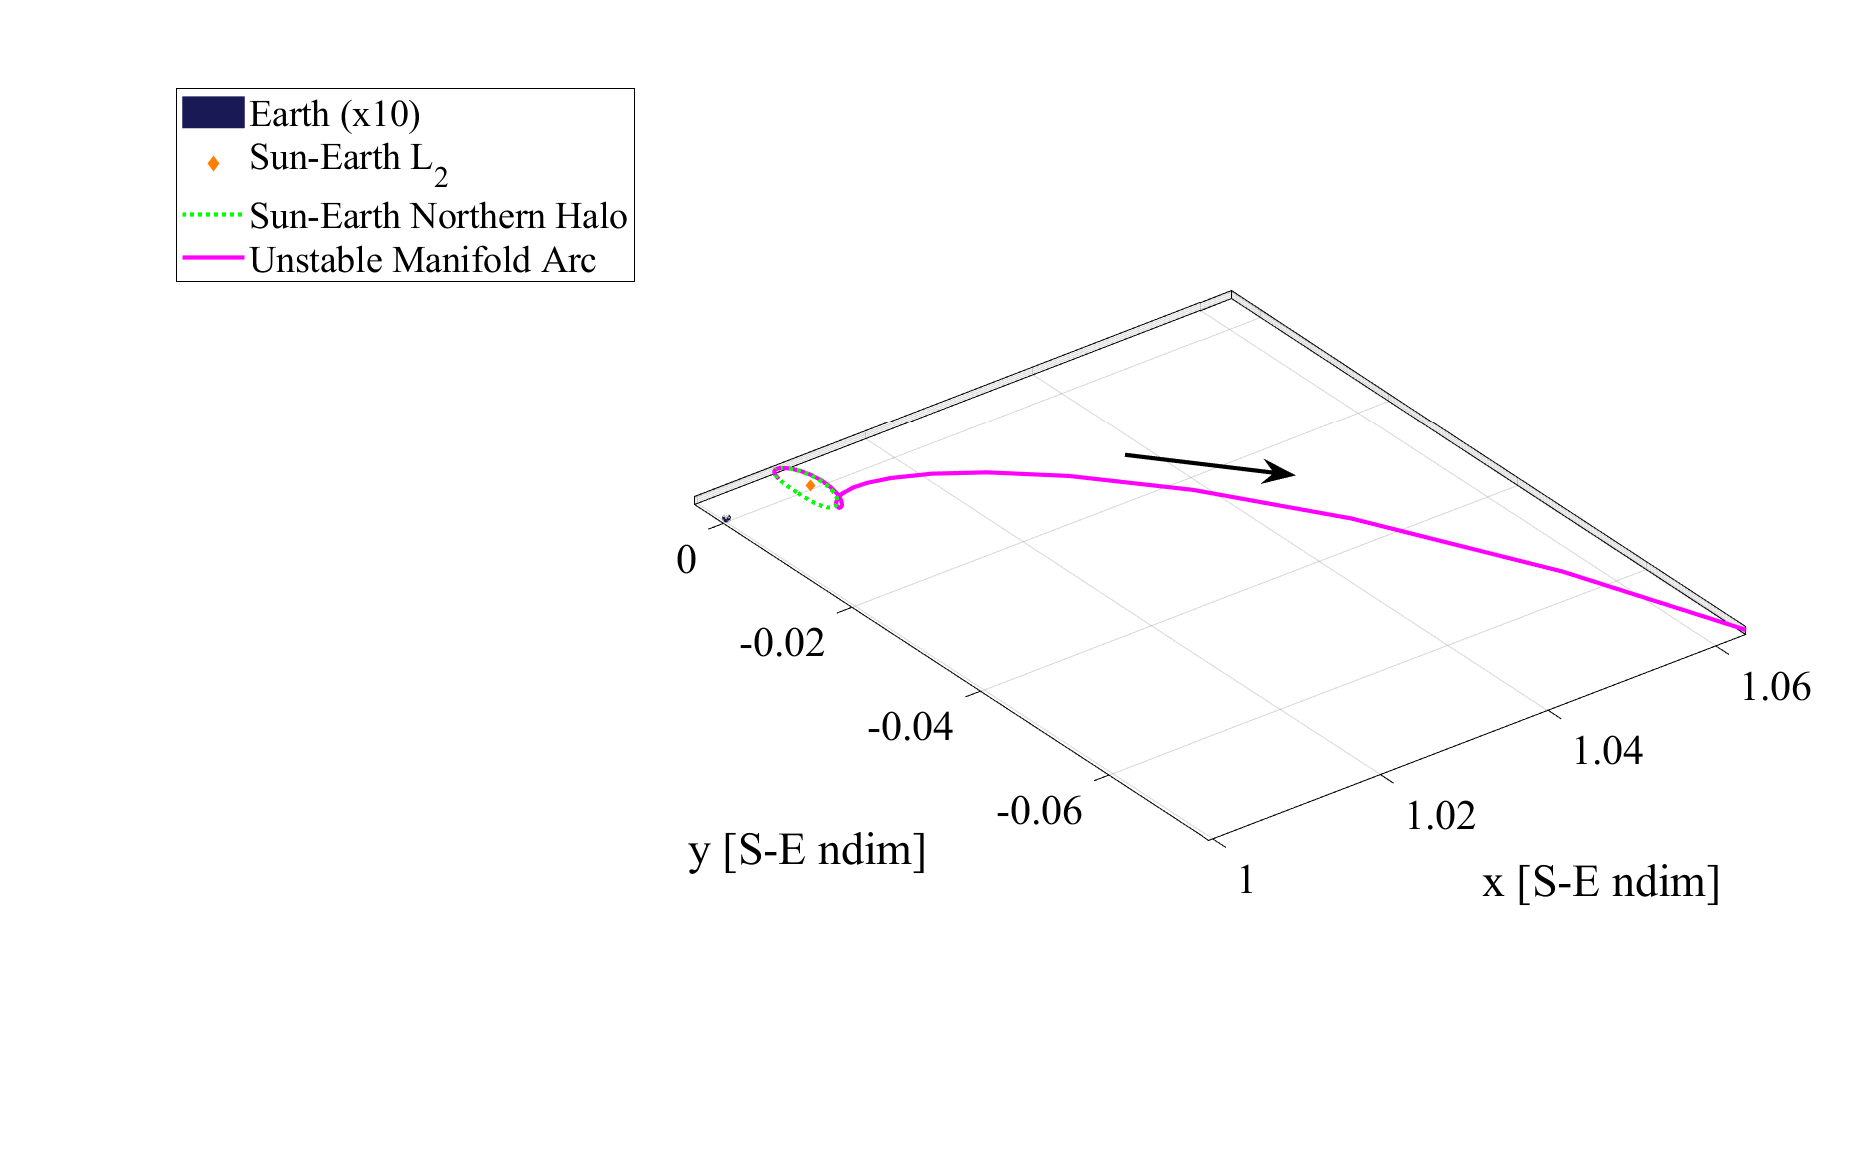
\includegraphics[width=0.9\textwidth]{figures/MinDvSE.pdf}
    \caption{MMAT departure CR3BP arc in the Sun-Earth barycentric rotating frame.}
    \label{fig:MMATSE}
\end{figure}

\begin{figure}[ht]
    \centering
    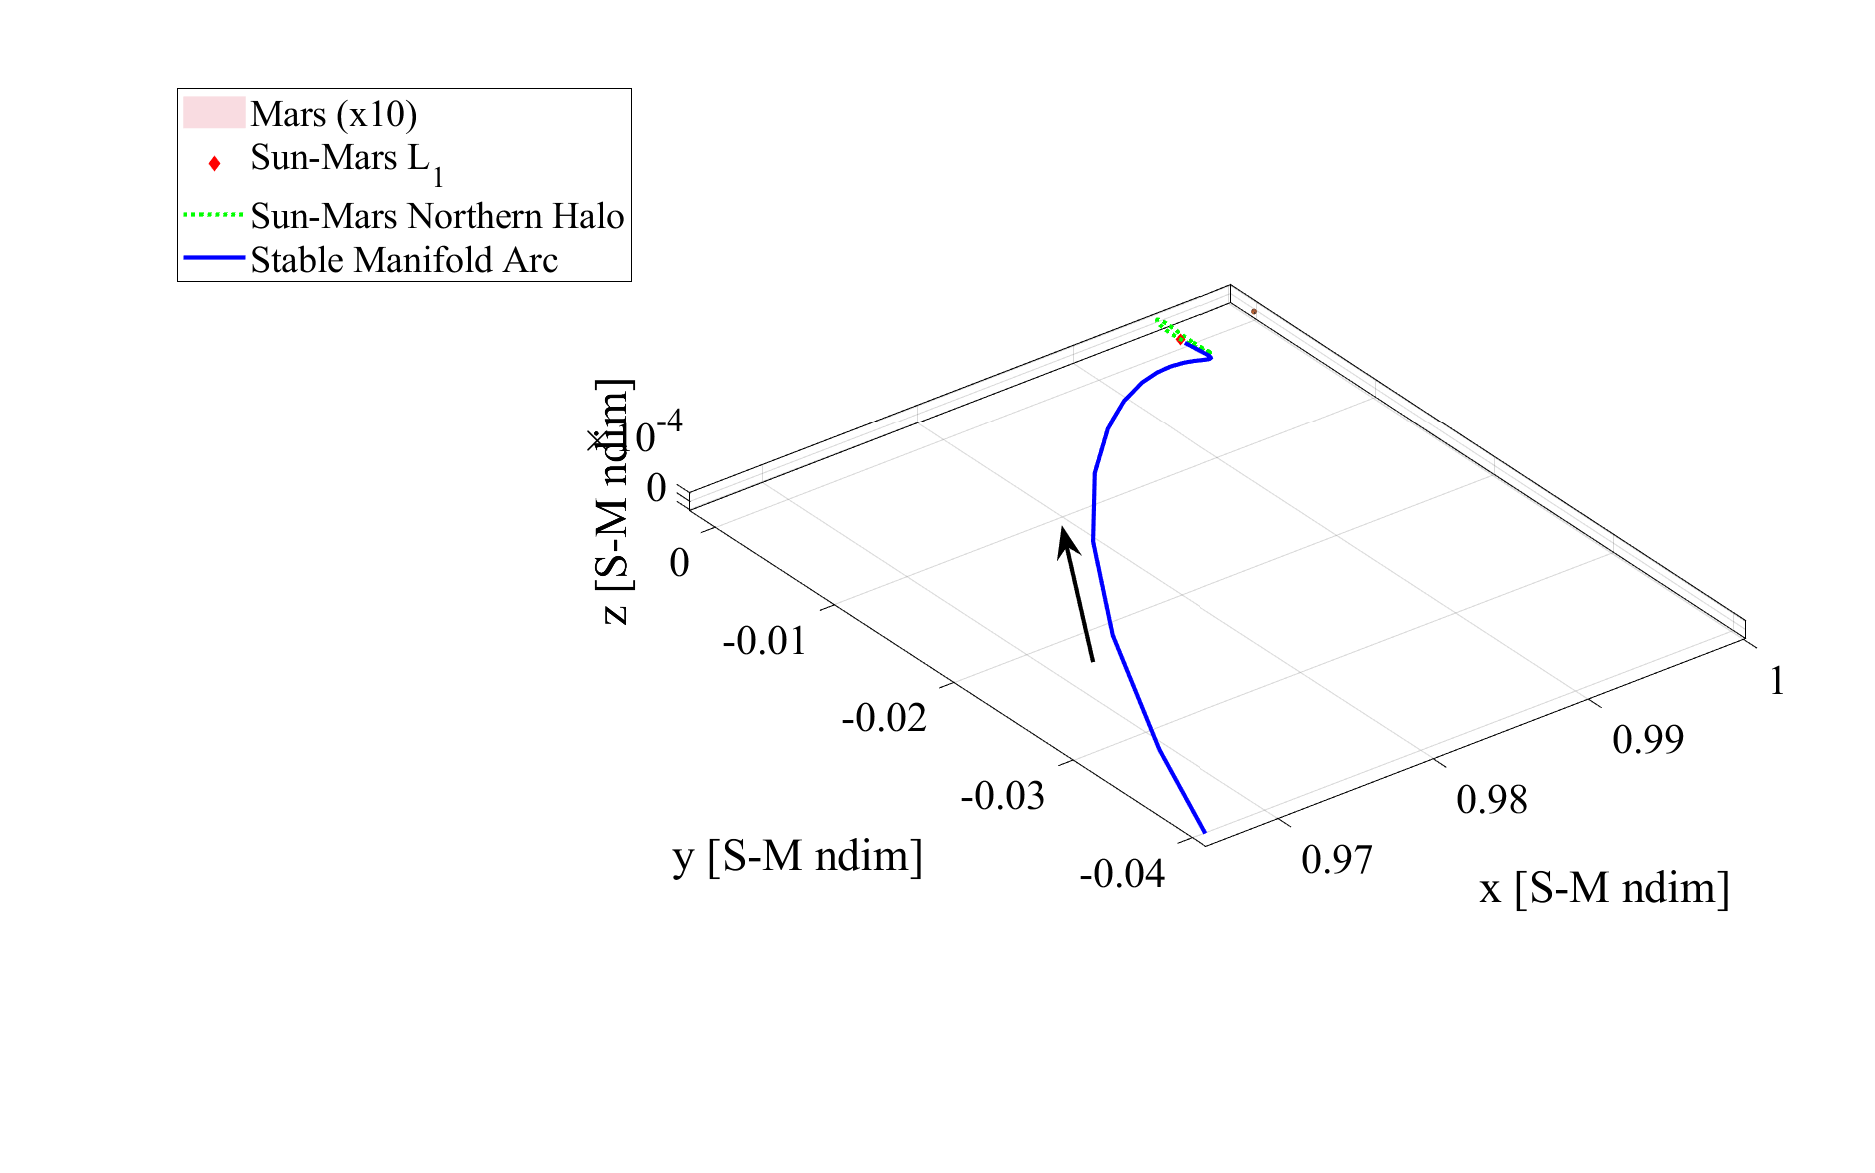
\includegraphics[width=0.9\textwidth]{figures/MinDvSM.pdf}
    \caption{MMAT arrival CR3BP arc in the Sun-Mars barycentric rotating frame.}
    \label{fig:MMATSM}
\end{figure}

In \cref{fig:MMATEvo}(a), the times-of-flight and maneuver magnitudes of the family members are
shown with respect to their initial phasing. Note that there are areas of initial epochs where
transfers could not be computed because the inequality in \cref{eq:MMAT} was not satisfied with
those orientations. Each successful epoch also has two transfer solutions corresponding to the two
arrival phasing solutions described above. The two groups of transfers in the figure correspond to 
the solutions where $n=0$ or $n=1$ satisfy \cref{eq:MMAT} and are similar because of symmetry
perpendicular to the intersection line of the Earth and Mars orbital planes. The full
time-of-flight for the transfers is generally bounded between 3 and 5 years, while the magnitude of
the two maneuvers combined is between 4 and 7 km/s.

\cref{fig:MMATEvo}(b) shows the same transfers, now with the required initial Mars phasing
$\theta_{0_{Mars}}$. This plot can be used to associate each transfer with an actual launch date
where the Earth and Mars are in the specified locations in their respective orbits. Varying the
chosen manifold departure arc while keeping the initial epoch fixed creates families that would
appear as vertical lines in \cref{fig:MMATEvo}(b), providing additional launch date flexibility but
potentially at the cost of maneuver $\Delta v$.

\begin{figure}[ht]
    \begin{subfigure}[h]{0.495\linewidth}
        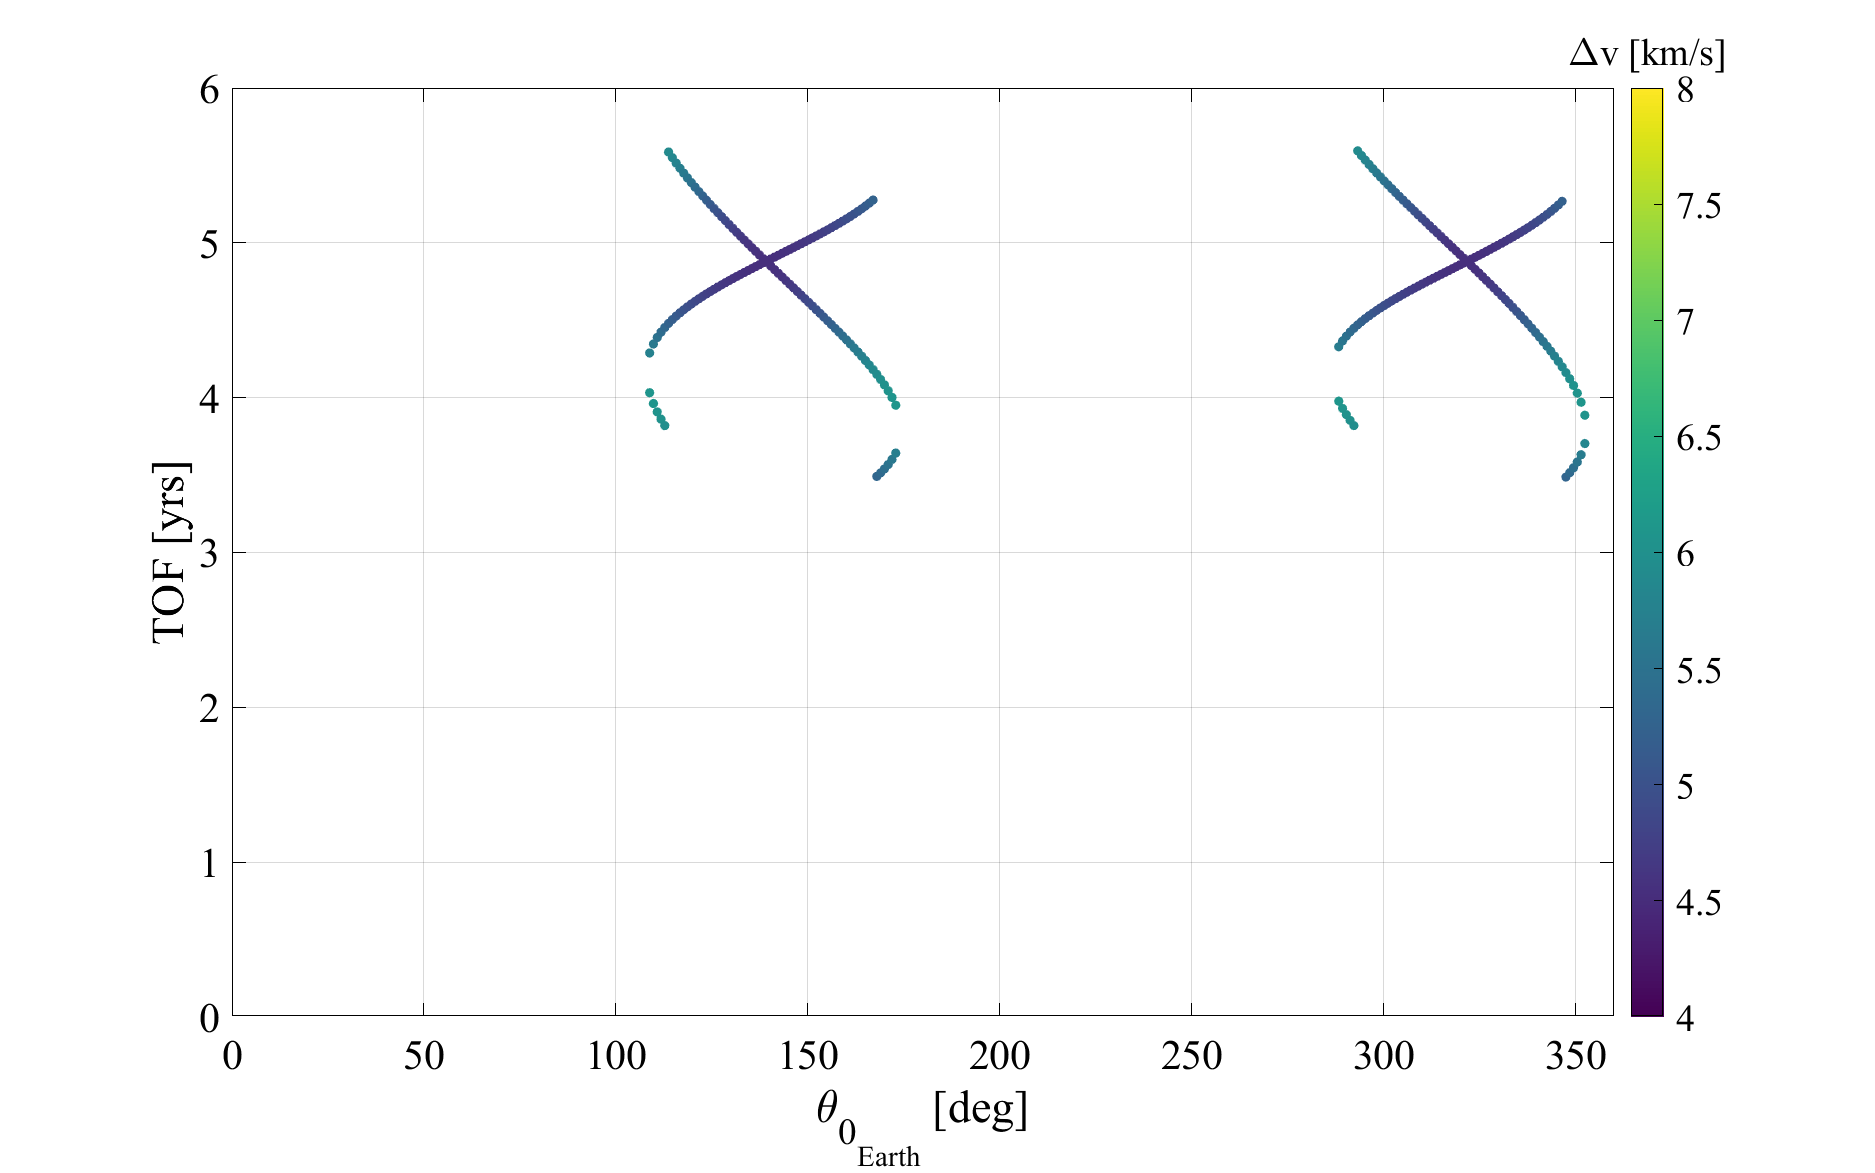
\includegraphics[width=\textwidth]{figures/MMATTOF.pdf}
        \caption{TOF and $\Delta v$}
    \end{subfigure}
    \hfill
    \begin{subfigure}[h]{0.495\linewidth}
        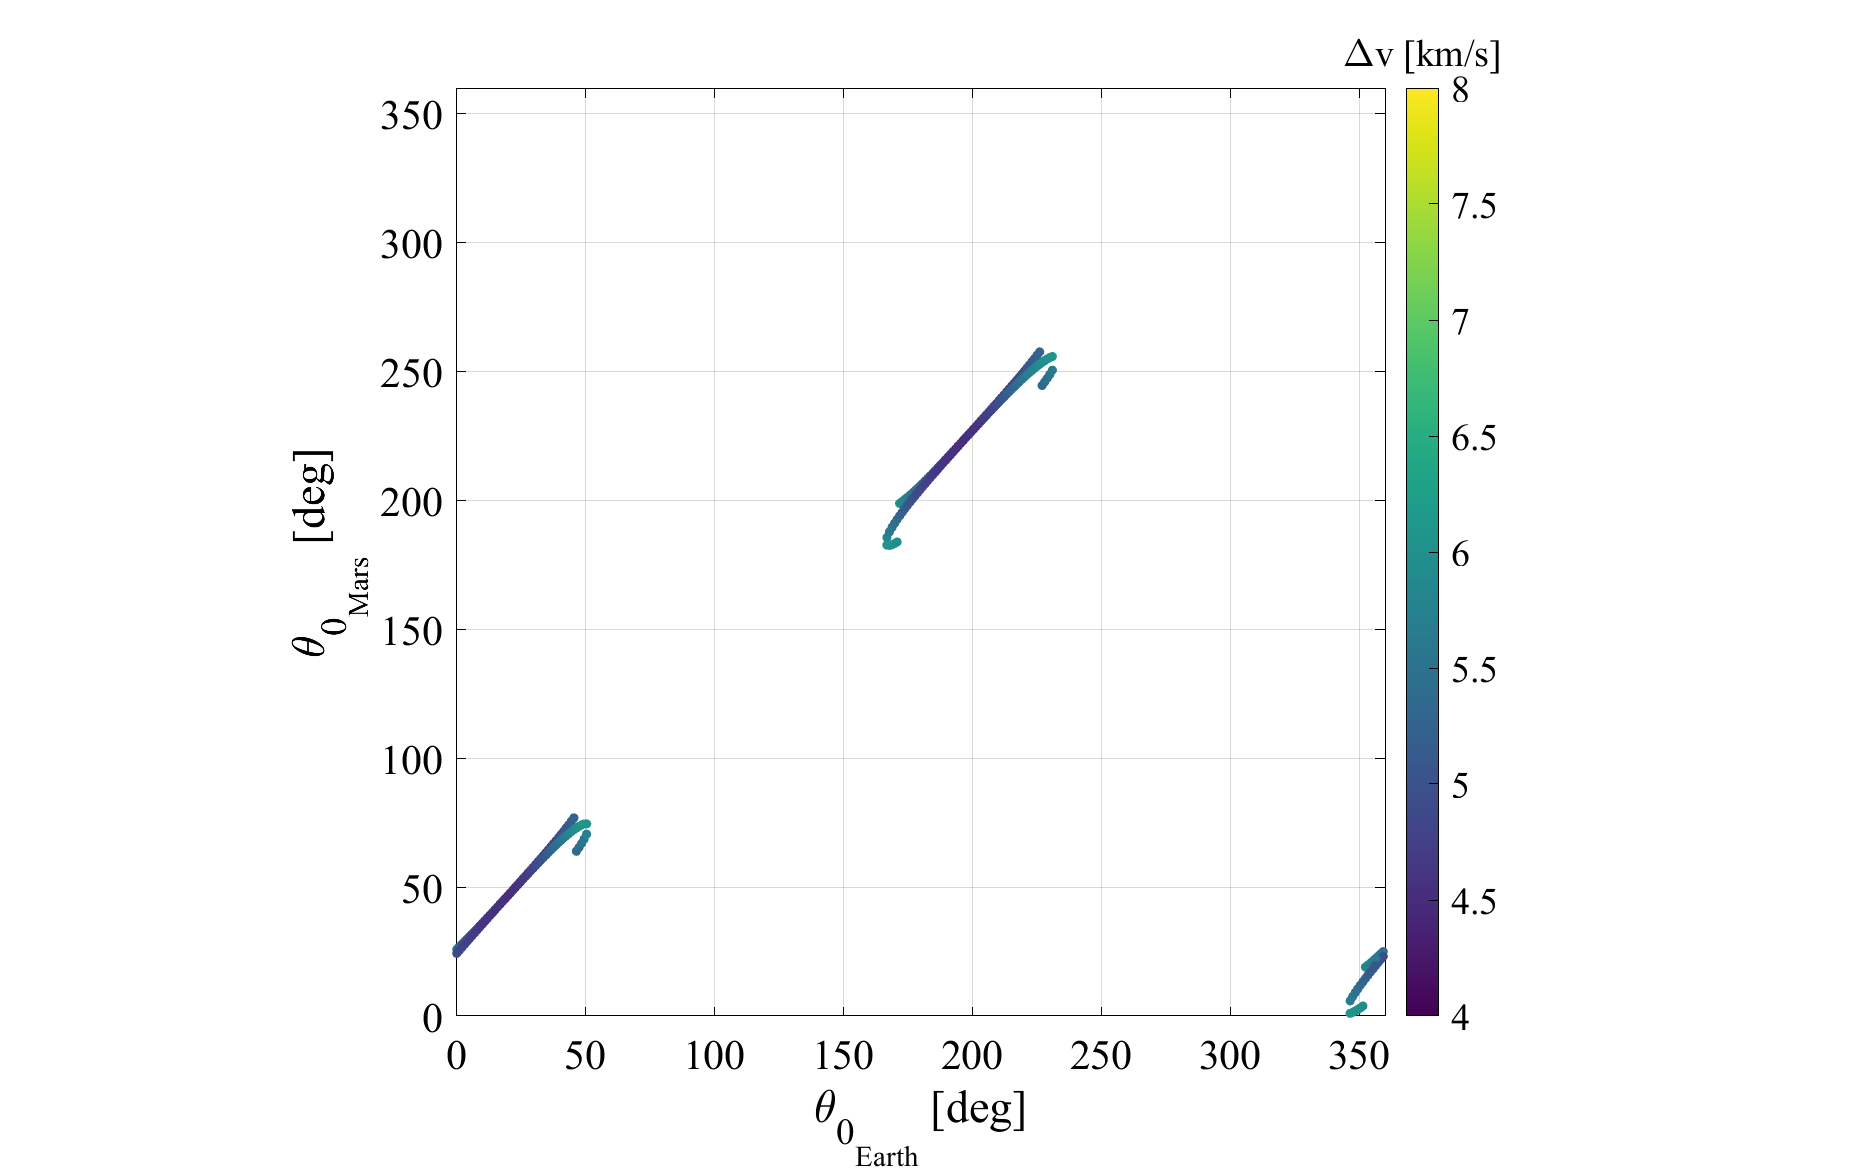
\includegraphics[width=\textwidth]{figures/MMATtheta.pdf}
        \caption{Required planet phasing}
    \end{subfigure}
    \caption{Evolution along the MMAT family continued by the initial epoch.}
    \label{fig:MMATEvo}
\end{figure}

The minimum-$\Delta v$ transfer from this family is shown in \cref{fig:MMATDv}. The total TOF of
the transfer is $1579$ days or $4.32$ years, with a total $\Delta v$ of $4.537$ km/s. In the
figure, the various arcs of the MMAT method are color-coded and the maneuvers are marked at the
beginning and end of the bridge conic arc. Note that the magenta departure CR3BP arc and the blue
arrival CR3BP arc are the same trajectories from \cref{fig:MMATSE} and \cref{fig:MMATSM}
respectively, just portrayed in the inertial frame. This transfer can be compared with the
minimum-TOF transfer in \cref{fig:MMATTOF}. This transfer has a different initial epoch, which
shifts all of the arcs, and a much shorter arrival conic arc. The total TOF has decreased to $1078$
days or $2.95$ years, but the $\Delta v$ has increased to $5.344$ km/s. Note that the first
maneuver has the same magnitude; the increase comes from the second maneuver where the minimum-TOF
burn is less tangential to the bridge arc than the minimum-$\Delta v$ burn to shorten the arrival
conic arc time-of-flight. All of the other transfers in this family have similar geometries and
characteristics.

\begin{figure}[ht]
    \centering
    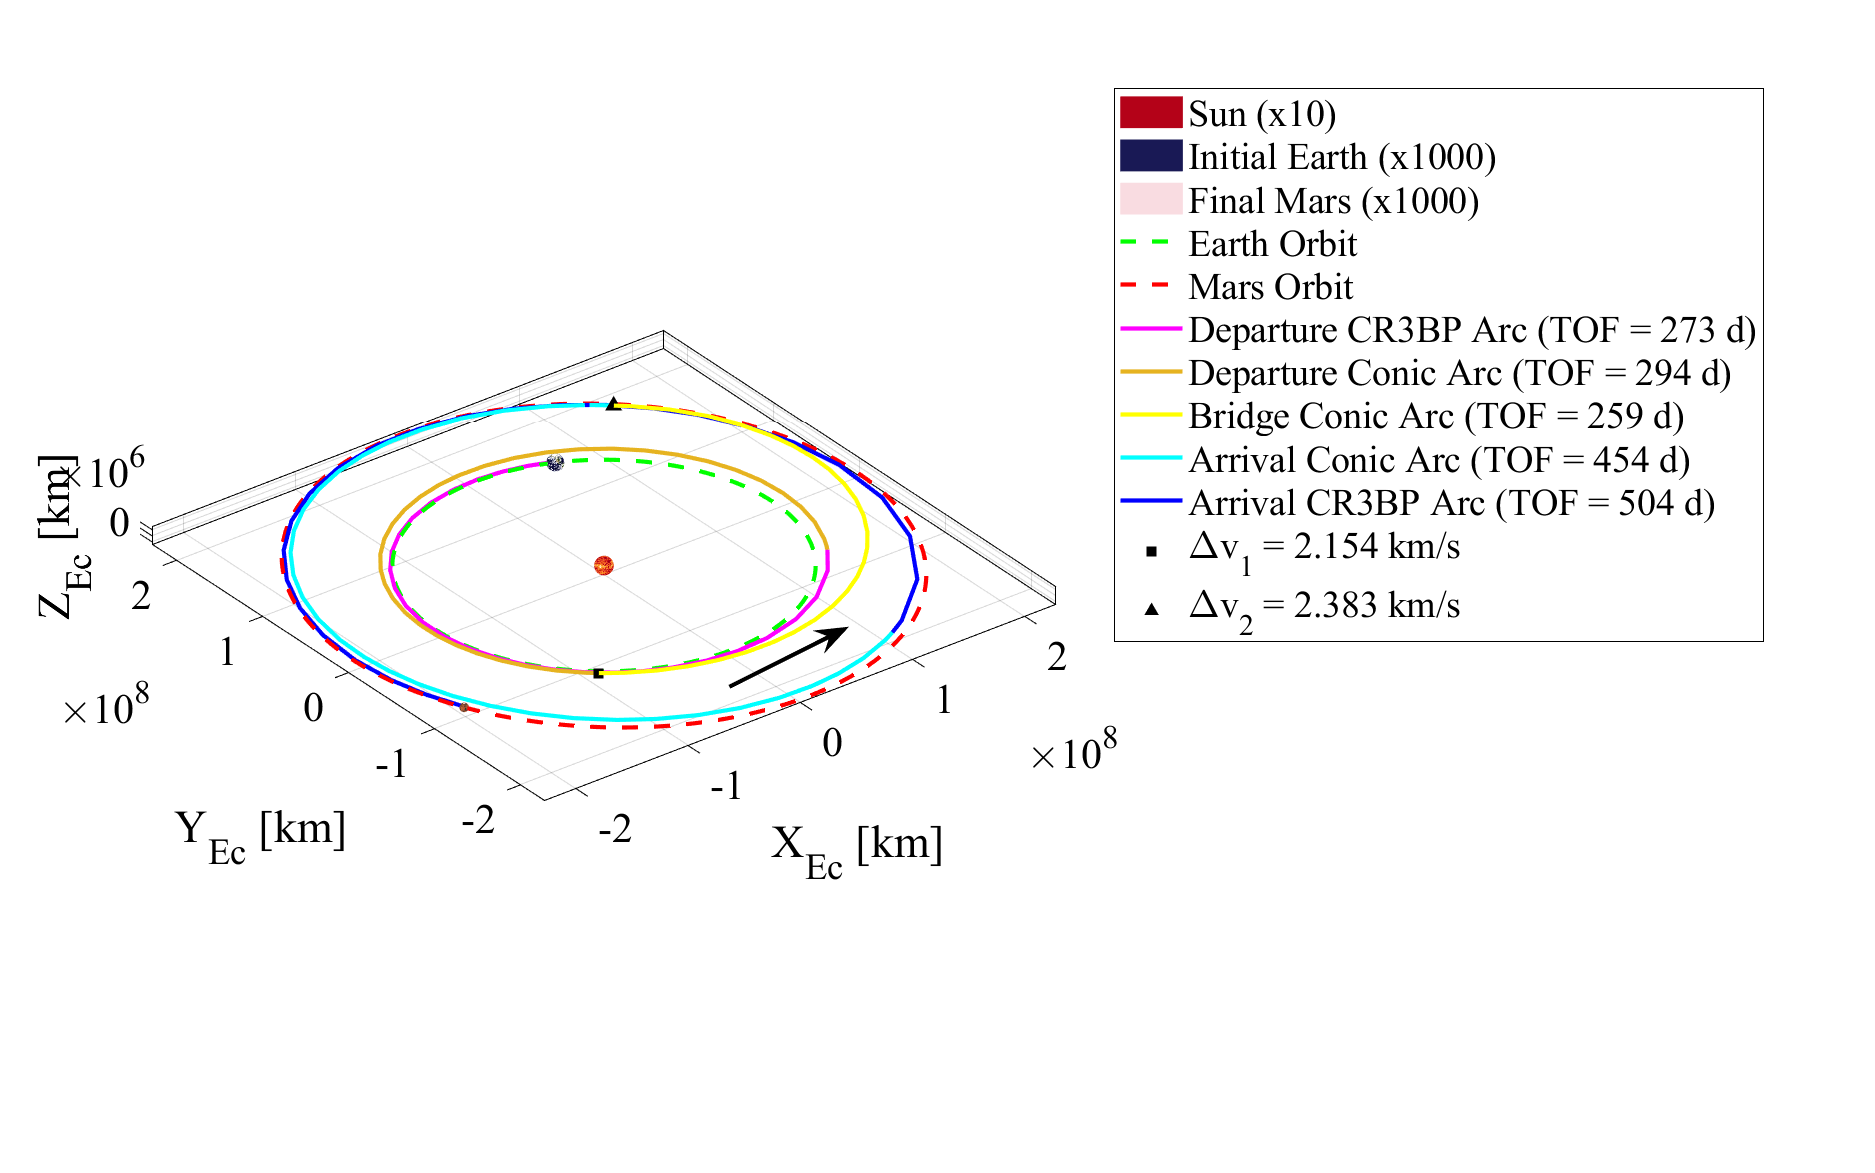
\includegraphics[width=0.9\textwidth]{figures/MinDvMMAT.pdf}
    \caption{Minimum-$\Delta v$ MMAT in the Sun-centered Ecliptic J2000 frame.}
    \label{fig:MMATDv}
\end{figure}

\begin{figure}[ht]
    \centering
    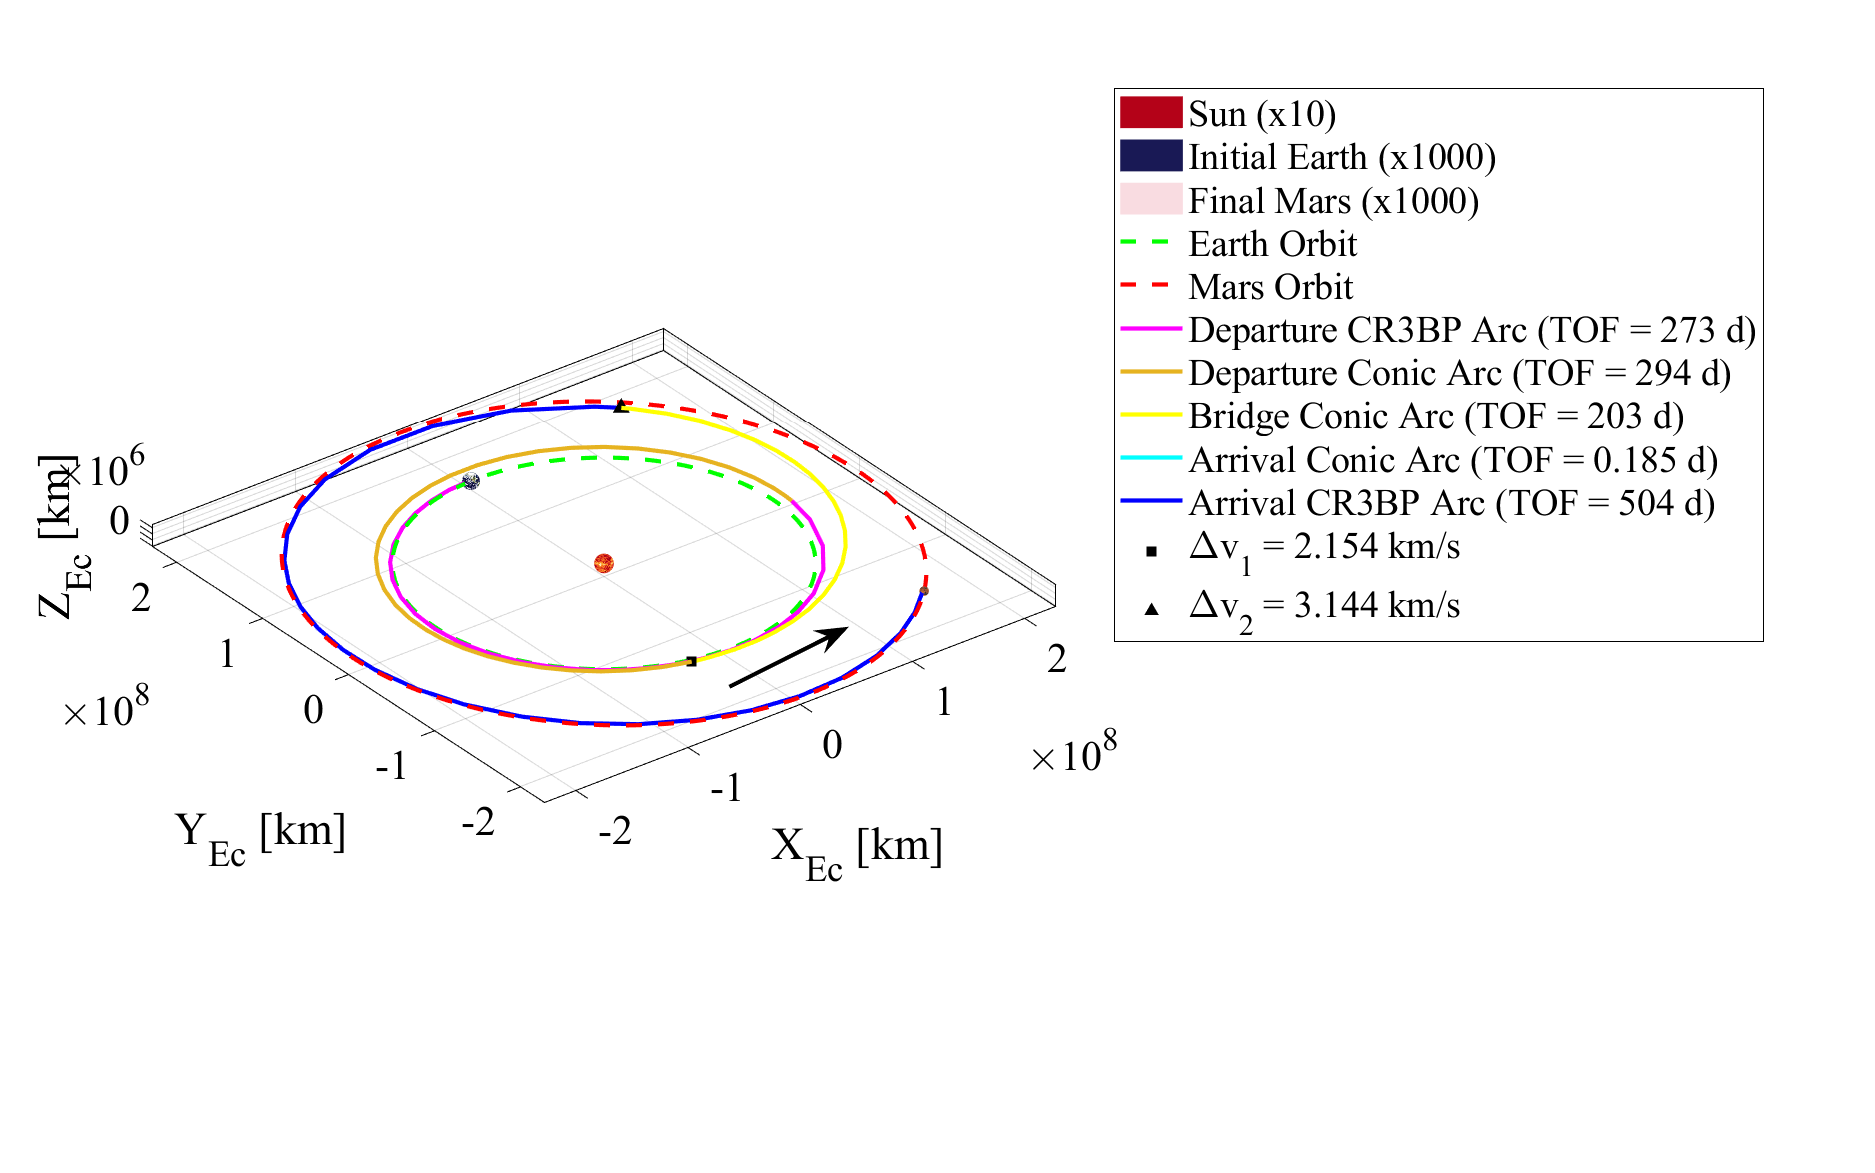
\includegraphics[width=0.9\textwidth]{figures/MinTOFMMAT.pdf}
    \caption{Minimum-TOF MMAT in the Sun-centered Ecliptic J2000 frame.}
    \label{fig:MMATTOF}
\end{figure}
